
\textbf{\underline{Третья глава}} посвящена разработке и исследованию преобразователя силы на основе Velostat собственного изготовления.

Для определения геометрических и физико-механических свойств поверхности было решено использовать датчик силы на ноге робота. Рассмотрев различные варианты, по причине отличного соотношения цены и получаемого результата, необходимо использовать пьзорезистивный тип датчика, основанный на материале Velostat \pic{fig:velostat_sensor.jpg}. Он является промежуточным слоем \pic{fig:simplest_sensor.jpg}. Электрическая схема \pic{fig:el_scheme}. 


\begin{figure}[ht]
    \begin{subfigure}[t]{0.33\textwidth}
        \centering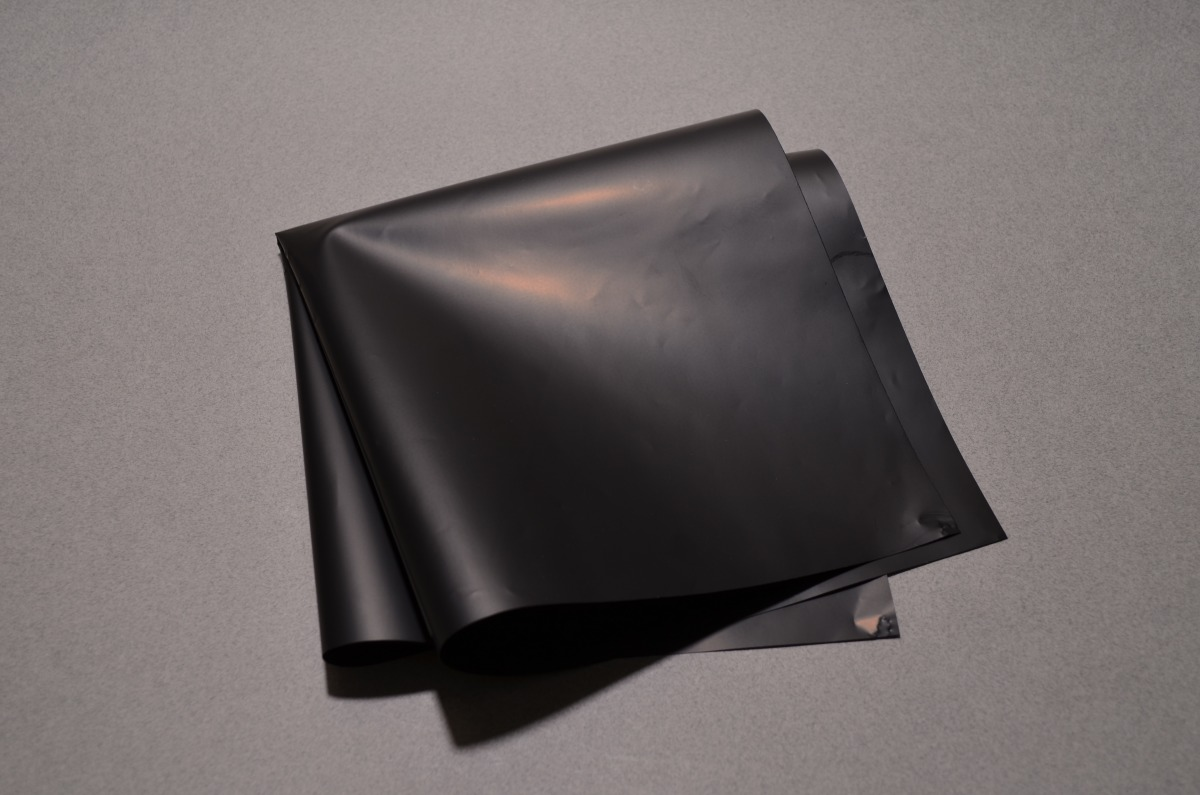
\includegraphics[height=2.5cm,width=1\textwidth,keepaspectratio]{velostat_sensor.jpg}
        \caption{Материал Velostat}
        \label{fig:velostat_sensor.jpg}
    \end{subfigure}
    \begin{subfigure}[t]{0.33\textwidth}
        \centering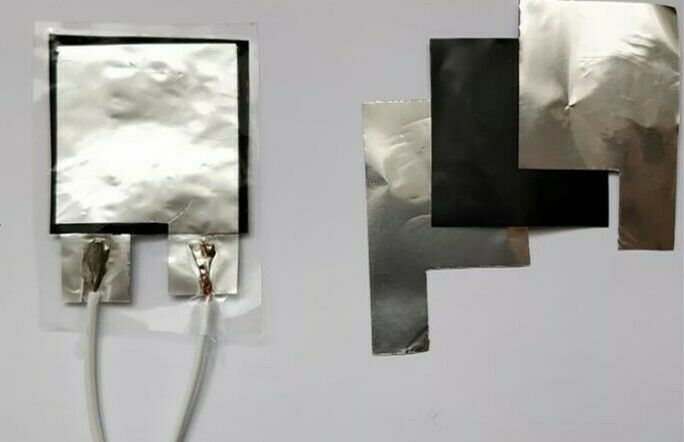
\includegraphics[height=2.5cm,width=1\textwidth,keepaspectratio]{simplest_sensor.jpg}
        \caption{Простейший преобразователь силы на основе Velostat}
        \label{fig:simplest_sensor.jpg}
    \end{subfigure}
    \begin{subfigure}[t]{0.33\textwidth}
        \centering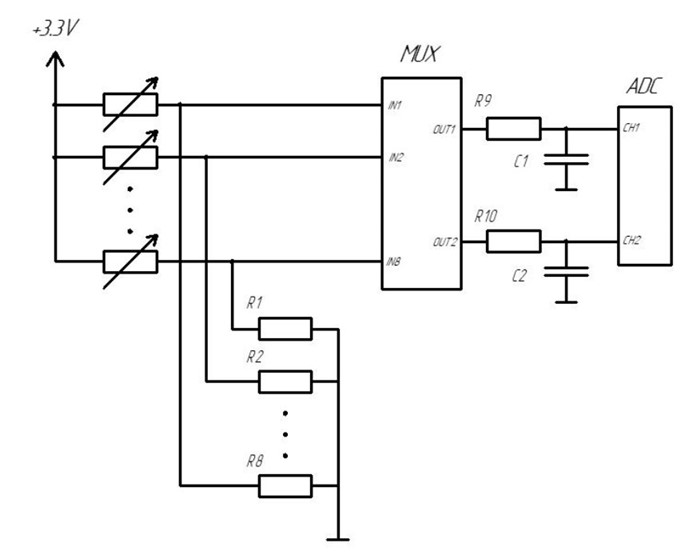
\includegraphics[height=4cm,width=1\textwidth,keepaspectratio]{electric_scheme.jpg}\\
        \caption{Электрическая схема преобразователя силы}
        \label{fig:el_scheme}
    \end{subfigure}
    \caption{Примеры использования Velostat}
\end{figure}

При исследовании преобразователя силы на основе Velostat, было замечено, что площадь нажатия влияет на показания преобразователя, поэтому возникла необходимость исследовать характеристики материала для случаев, когда площадь приложения силы меньше чем площадь активной части сенсора.

Исследования сенсора выполнялись на специально разработанном для этого стенде. Требования: необходимость контролировать силу нажатия и обеспечить повторяемость эксперимента как по величине, так и по расположению площадки контакта инструмента и исследуемого преобразователя силы. 

Разработанный стенд, представлен на рисунке \ref{fig:exp_standd}.

\begin{figure}[ht]
    \begin{center}
            \begin{tikzpicture}
                % Include the image in a node
                \node [
                    above right,
                    inner sep=0] (image) at (0,0) {\centering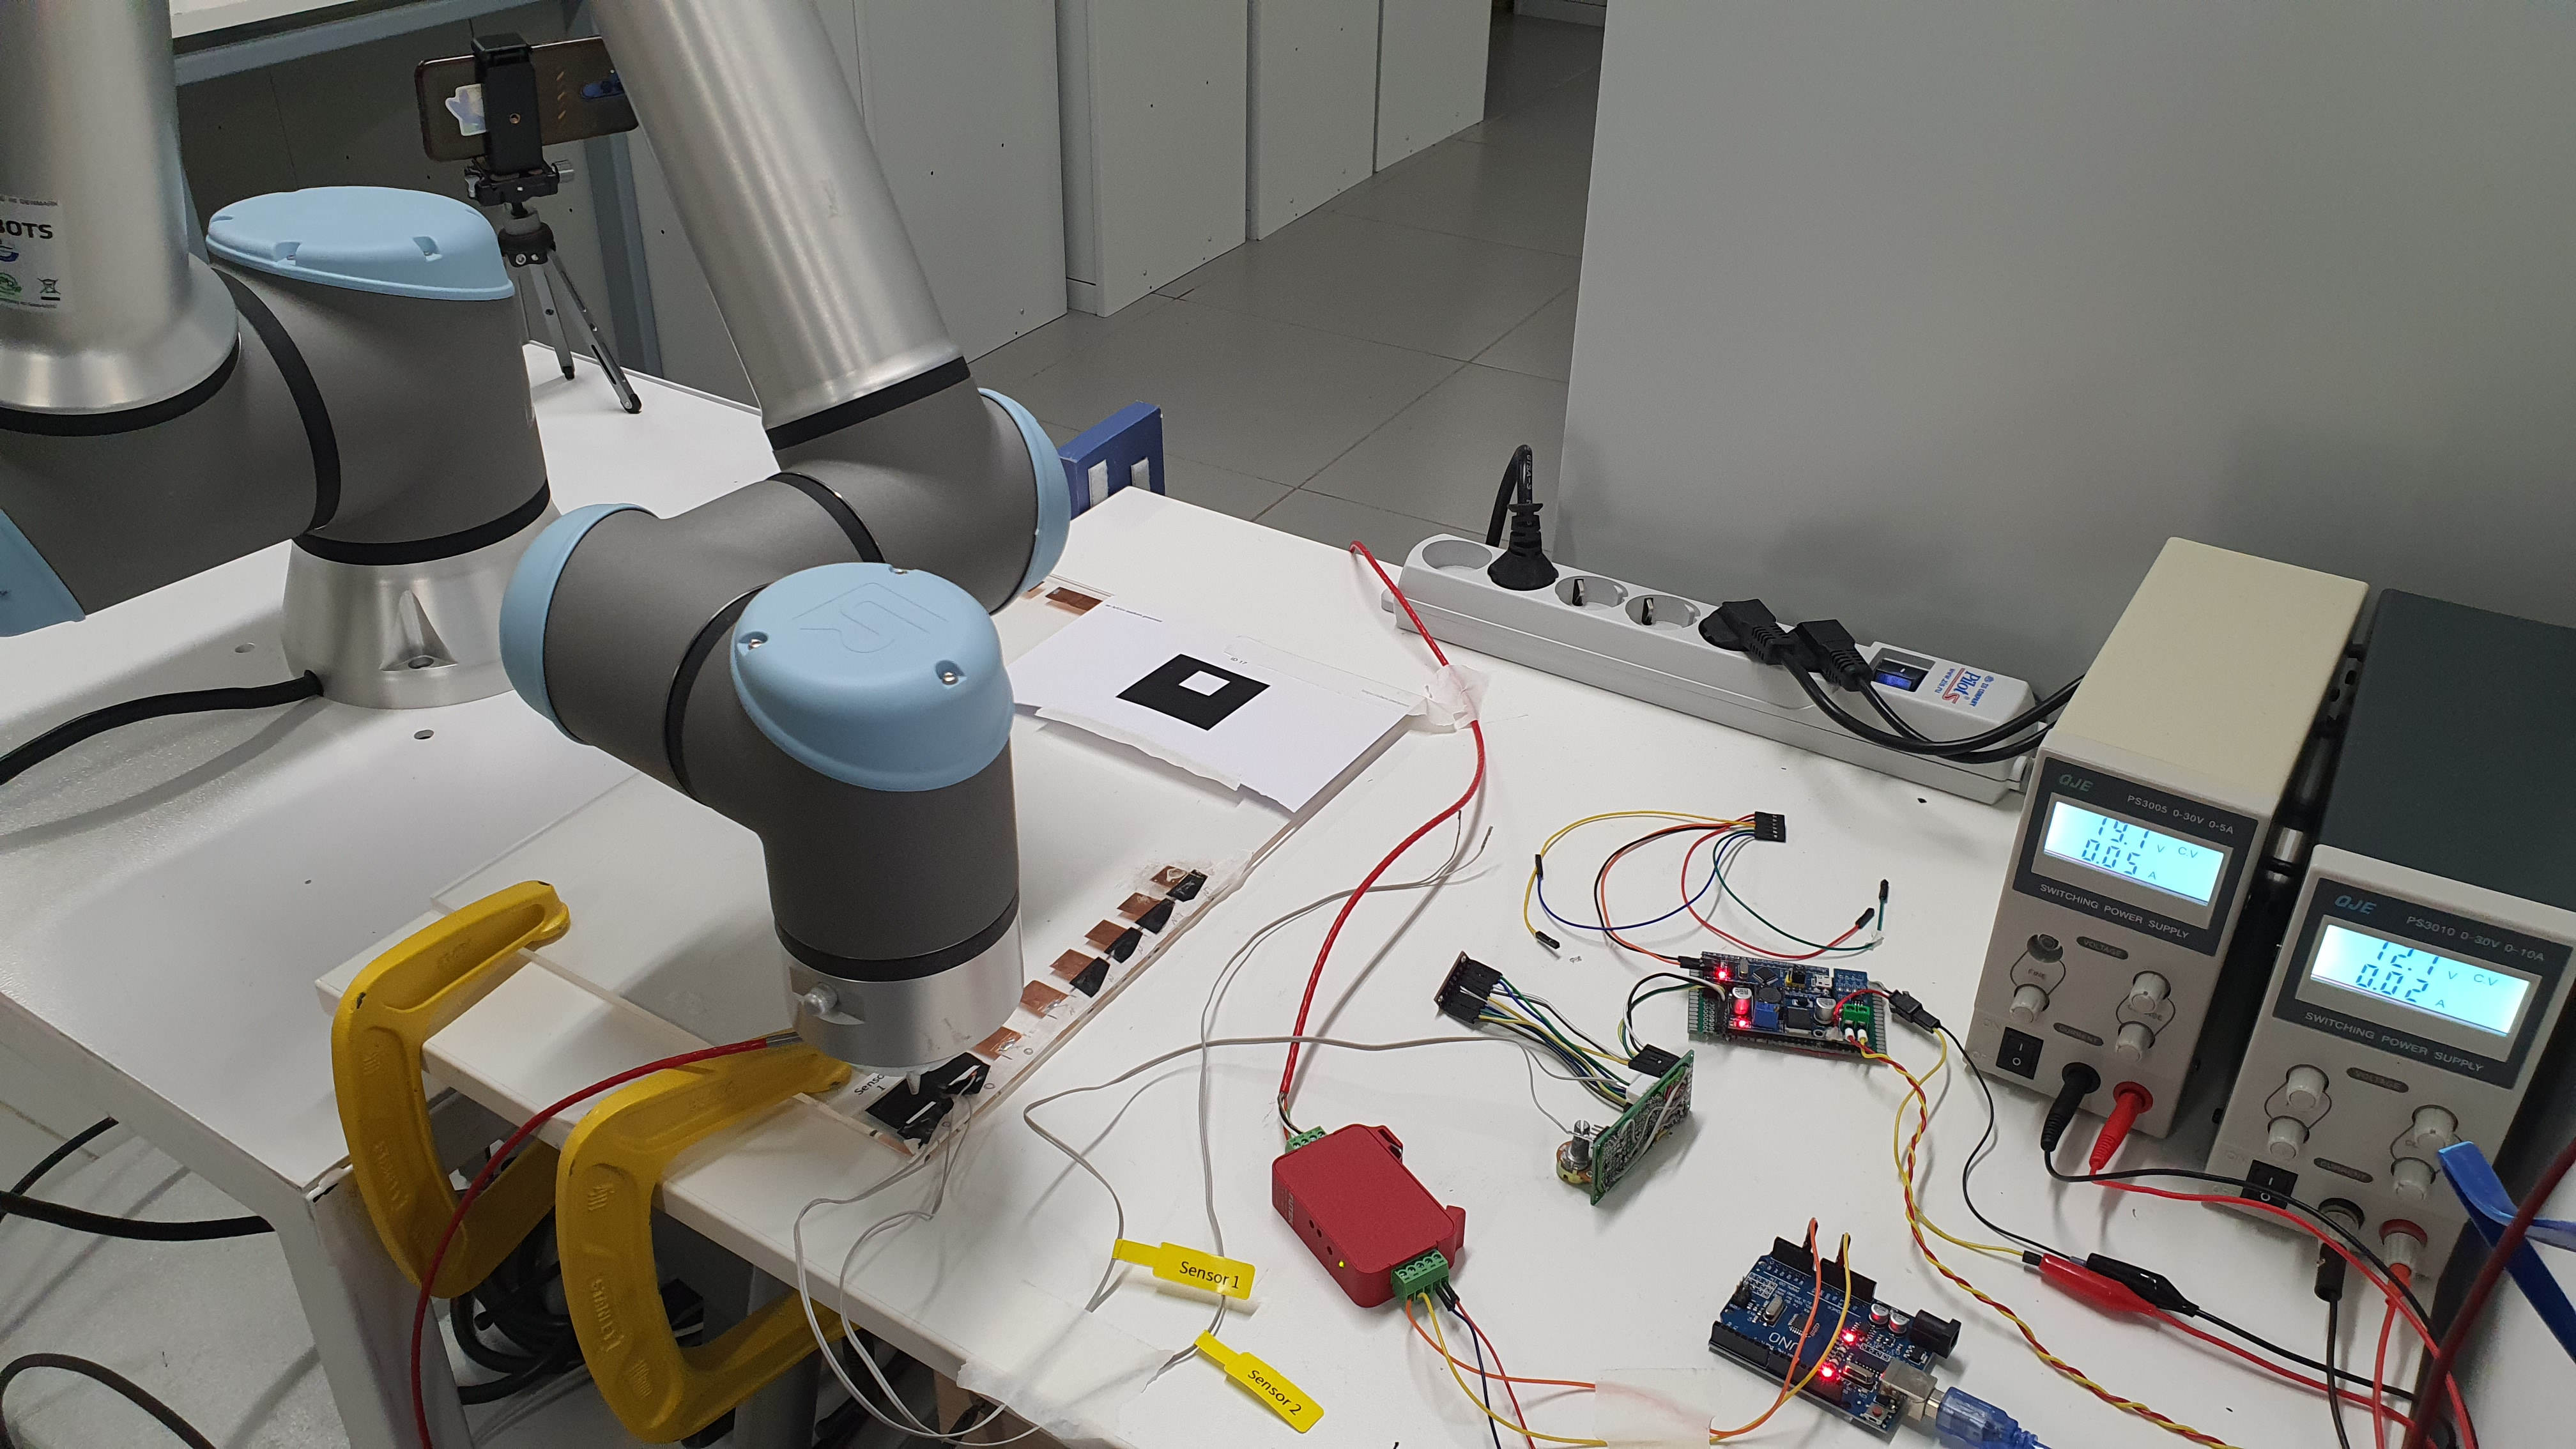
\includegraphics[height=5cm,width=1\textwidth,keepaspectratio]{exp_stand1}};

                % Create scope with normalized axes
                \begin{scope}[
                        x={($0.1*(image.south east)$)},
                        y={($0.1*(image.north west)$)}]
                    \draw[latex-, very thick,green] (3.5,2.2) -- (2.5,1)
                    node[rounded corners=3pt,below left,black,fill=white]{\small Velostat сенсор};

                    \draw[stealth-, very thick,green] (3.5,2.6) -- ++(-0.7,+0.5)
                    node[rounded corners=3pt,left,black,fill=white]{\small Датчик силы};

                    \draw[stealth-, very thick,green] (6.5,3) -- (7,6)
                    node[rounded corners=3pt,above right,black,fill=white]{\small Self-made PCB};

                    \draw[stealth-, very thick,green] (7.2,1.5) -- (8,5)
                    node[rounded corners=3pt,above right,black,fill=white]{\small Ардуино};

                    \draw[stealth-, very thick,green] (2.5,9.5) -- (4,9.5)
                    node[rounded corners=3pt,right,black,fill=white]{\small Камера};

                    \draw[very thick,green] (0.5,2.5) rectangle (4.2,9)
                    node[below left,black,fill=green]{\small UR10e};

                    \draw[latex-, very thick,green] (4.5,7.2) edge (5.5,7.5)
                    (4.8,5.3) -- (5.5,7.5)
                    node[rounded corners=3pt,above,black,fill=white]{\small Aruco маркеры};
                \end{scope}
            \end{tikzpicture}
        
        \caption{Разработанный экспериментальный стенд}
        \label{fig:exp_standd}
    \end{center}
\end{figure}

Для касания только части объекта исследования были разработаны различные насадки. Минимальный размер препятствия, которого может коснуться робот, был принятым равным 2 мм. Длина ребра датчика -- 15 мм \pic{fig:all_end_effectors.png}.

\begin{figure}[ht]
    \begin{subfigure}{0.6\textwidth}
        \centering
        \begin{tikzpicture}
            % Include the image in a node
            \node [above right, inner sep=0] (image) at (0,0)
            {\centering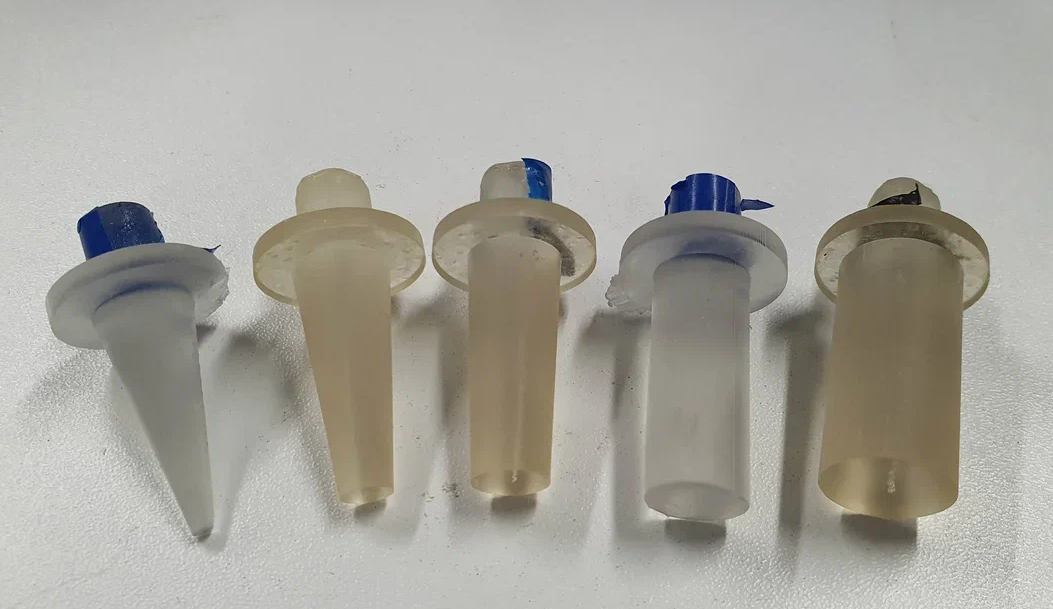
\includegraphics[height=3.5cm,width=1\textwidth,keepaspectratio]{all_end_effectors.png}};
            % Create scope with normalized axes
            \begin{scope}[
                    x={($ 0.1*(image.south east)$)},
                    y={($ 0.1*(image.north west)$)}]
                \node[rounded corners=3pt,black,fill=white] at (1.1,7.4){\tiny 2 мм };
                \node[rounded corners=3pt,black,fill=white] at (3.1,7.9){\tiny 6 мм };
                \node[rounded corners=3pt,black,fill=white] at (4.9,8.1){\tiny 8 мм };
                \node[rounded corners=3pt,black,fill=white] at (6.7,7.9){\tiny 12 мм };
                \node[rounded corners=3pt,black,fill=white] at (8.6,7.9){\tiny 15 мм };
            \end{scope}
        \end{tikzpicture}
        \caption{Насадки для нажатия на сенсор}
        \label{fig:all_end_effectors.png}
    \end{subfigure}
    \begin{subfigure}{0.38\textwidth}
        \centering
        \begin{tikzpicture}

            % Include the image in a node
            \node [
                above right,
                inner sep=0] (image) at (0,0) {\centering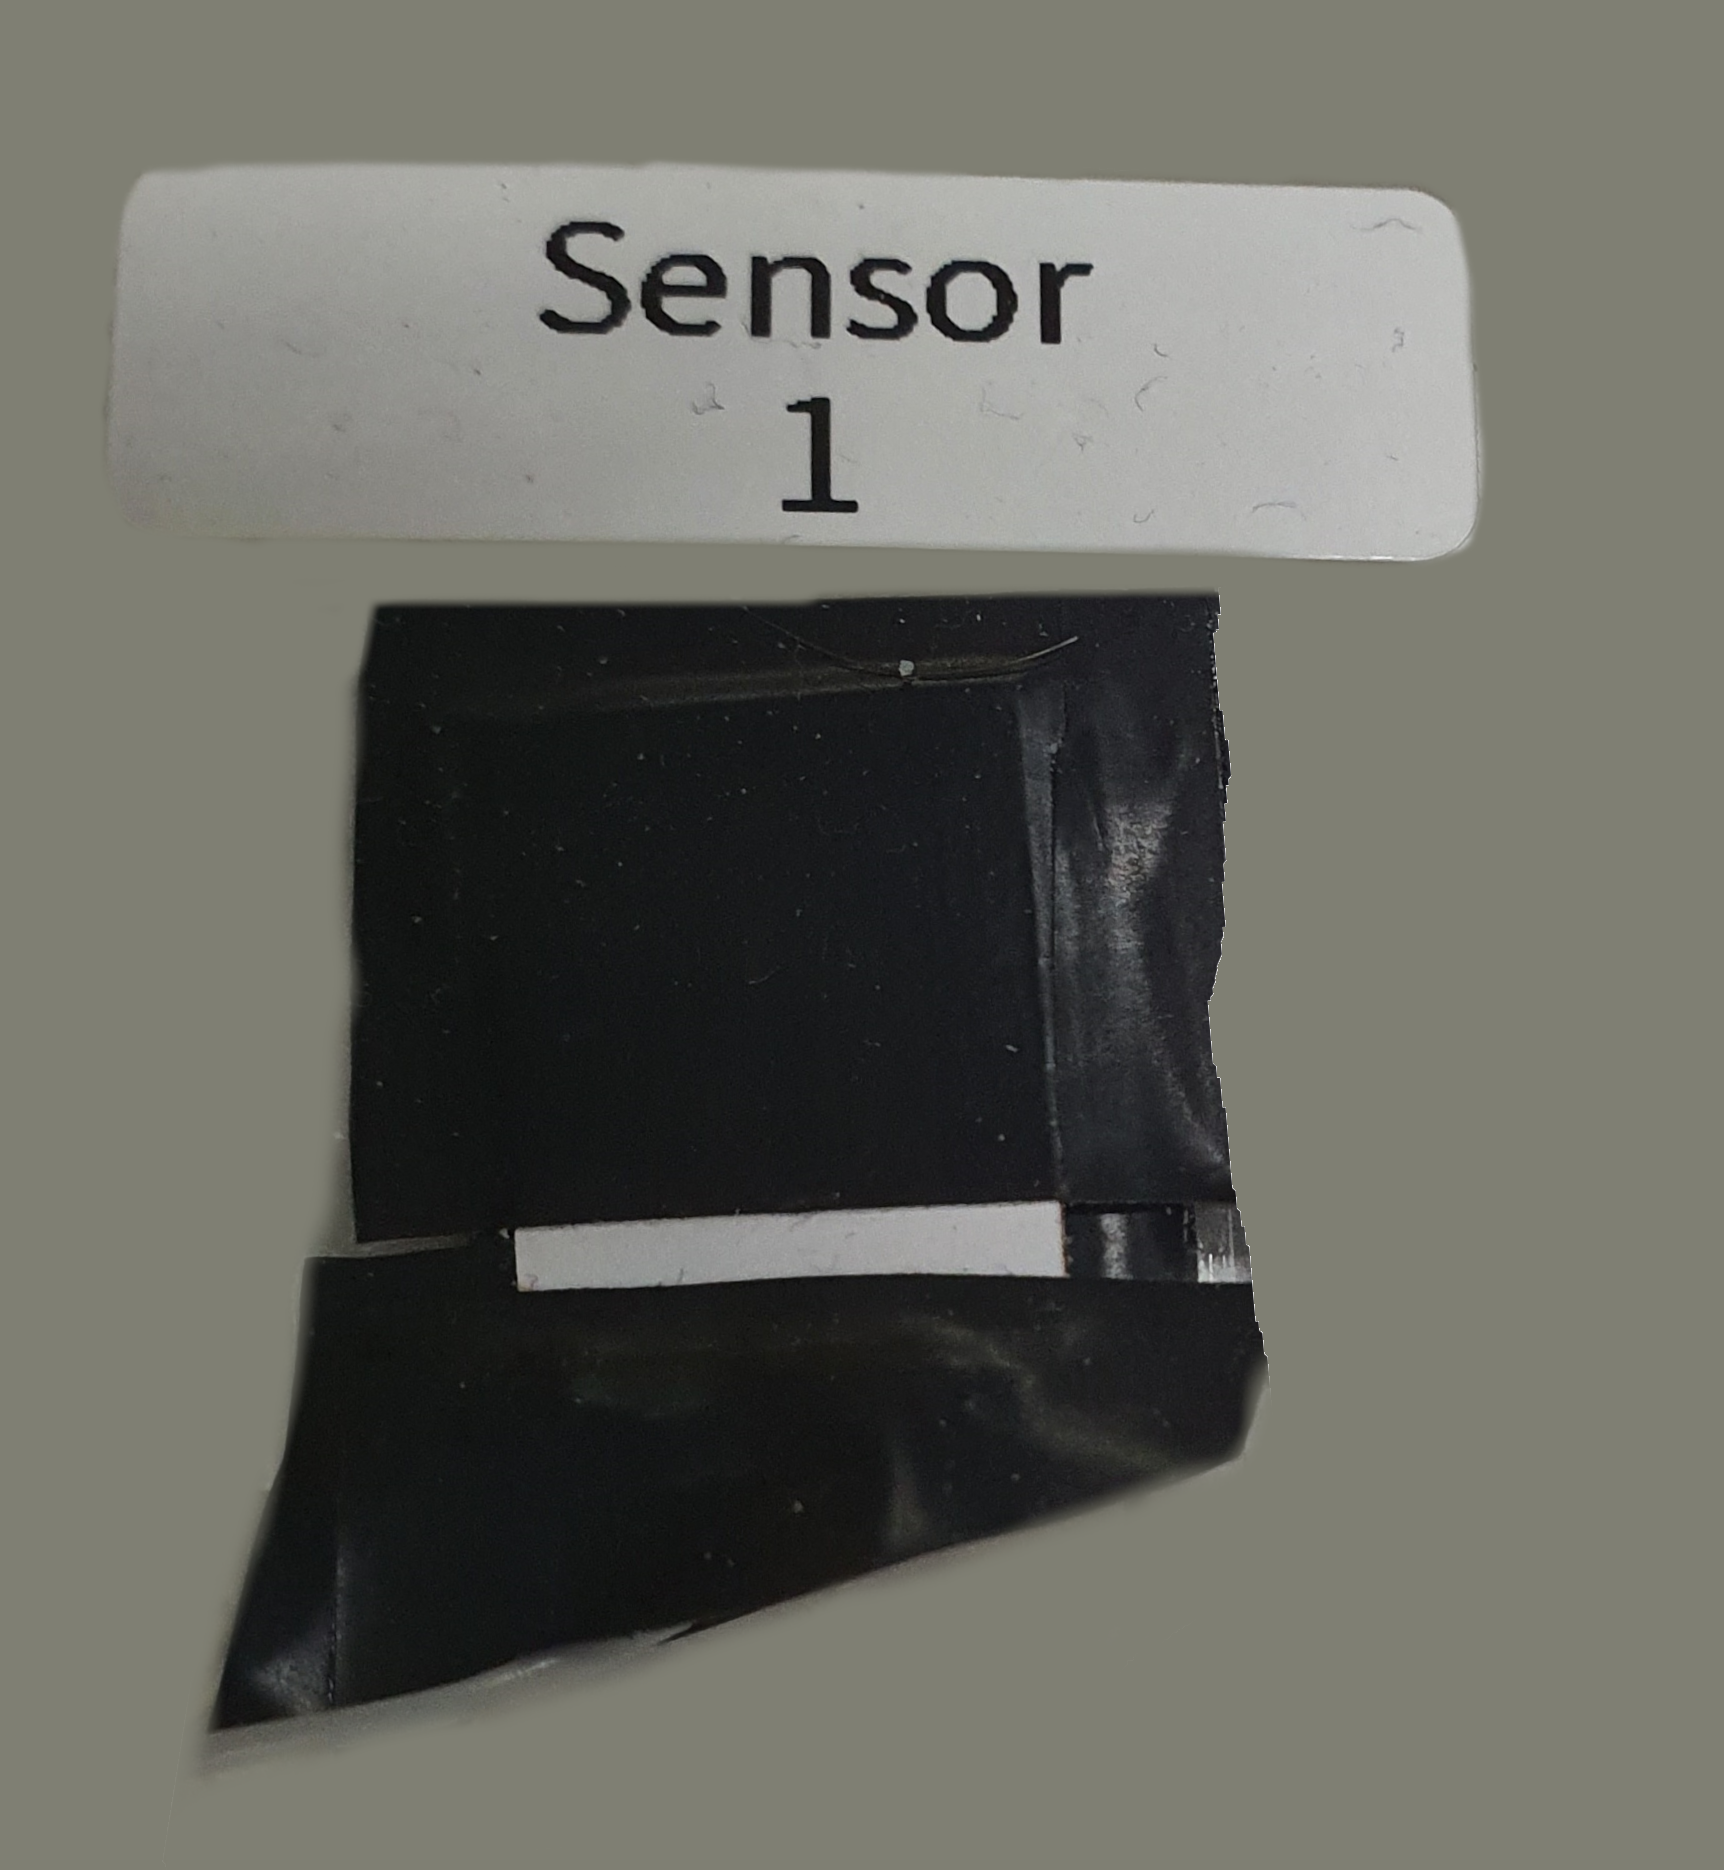
\includegraphics[height=3.5cm,width=1\textwidth,keepaspectratio]{sensors_grid.png}};

            % Create scope with normalized axes
            \begin{scope}[
                    x={($0.1*(image.south east)$)},
                    y={($0.1*(image.north west)$)}]
                \draw [green, very thick,
                    decorate,
                    decoration = {brace,
                            raise=5pt,
                            amplitude=5pt,
                            aspect=0.5}] (6,3.7) --  (3,3.7)
                node[pos=0.5,below=10pt,green]{$15$ мм};

                \draw [green, very thick,
                    decorate,
                    decoration = {brace, mirror,
                            raise=5pt,
                            amplitude=5pt,
                            aspect=0.5}] (6,3.6) --  (6,6.4)
                node[pos=0.5,right=10pt,green]{$15\ $ мм};

                \draw[green,step=1,xshift=22, yshift=30]  (0.5,0.5) grid +(3,3);

                \node[circle,fill=green,scale=0.4] at (3.3,6.27){\small 1};
                \node[circle,fill=green,scale=0.4] at (5.92,3.7){\small 16};
            \end{scope}

        \end{tikzpicture}
        \caption{Сенсор представлен \\ как $4\times4$ сетка}
        \label{fig:sensor_grid}
    \end{subfigure}
    \caption{Представление места нажатия инструментом сенсора и сам инструмент}
\end{figure}

Для контролирования силы нажатия манипулятором сенсора, было реализовано импедансное управления по оси, перпендикулярной плоскости датчика.

Было проведено два эксперимента: статический и динамический В \textbf{статическом} решалась задача определения коэффициентов для математической модели преобразователя (калибровка датчика). В рамках эксперимента на сенсор прикладывалась известная нагрузка на 60 секунд.

Для калибровки использовалась формула \eqref{eq:velostat_eqn}. Из-за гистерезиса необходимо учитывать время нажатия на объект, так как показания сенсора меняются со временем.
\begin{align}
    \label{eq:velostat_eqn}
    V_{out} = V_0 + p[k_p + k_e(1-e^\frac{-(t-t_0)}{\tau_{res}})](1-e^{-\frac{A}{p}}) \\
    k_p = A_1e^{-A_2p}; \tau_{res} = B_0 + B_1e^{-\frac{p}{B_2}}
\end{align}
где,  $V_0$- начальное напряжение; $p,\ A_i,\ B_i,\ \tau_{res},\ k_i$  - настраиваемые константы; $t$ - текущее время; $t_0$ - время начала нажатия.
Для решения задачи регрессии использовался робастный нелинейный алгоритм наименьших квадратов \pic{fig:least_square_model.png}.

\begin{figure}[H]
    \centering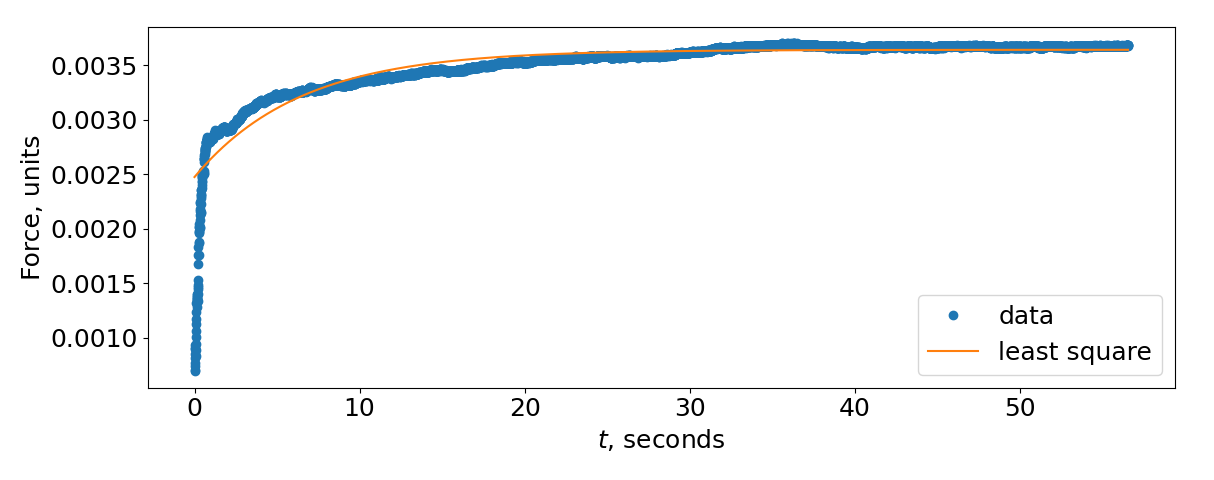
\includegraphics[height=3cm,width=1\textwidth,keepaspectratio]{least_square_model.png}
    \caption{Результаты статического эксперимента}
    \label{fig:least_square_model.png}
\end{figure}

\textbf{Динамический эксперимент}. Цель --- определить влияние показаний сенсора в зависимости от положения площадки контакта. Для этого преобразователь представлен в виде матрицы $4 \times 4$ \pic{fig:sensor_grid}. Манипулятор нажимает на преобразователь с одинаковым давлением на протяжении всех экспериментов в различные позиции на преобразователе, используя последовательно пять насадок \pic{fig:all_end_effectors.png}.



Результаты распределения ошибок по площади сенсора при взаимодействии с насадками разных размеров \pic{fig:dynamics_exp}. Ошибки определялись как разница между нормализованными показаниями калиброванного сенсора силы Futek и исследуемого преобразователя на базе Velostat.

\begin{figure}[H]
    \begin{subfigure}{0.49\textwidth}
        \centering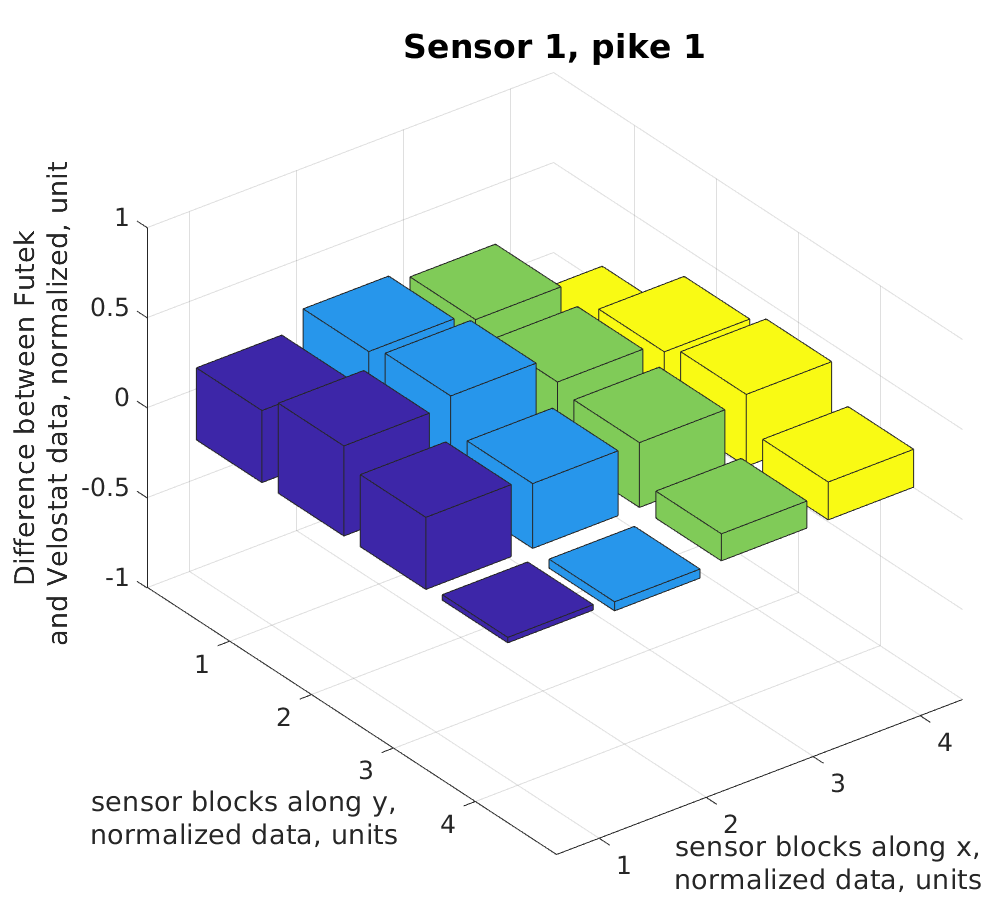
\includegraphics[height=5cm,width=1\textwidth,keepaspectratio]{sens1_pike1.png}
        \caption{Диаметр насадки равный 2 мм }
        \label{fig:sens1_pike1}
    \end{subfigure}
    \begin{subfigure}{0.49\textwidth}
        \centering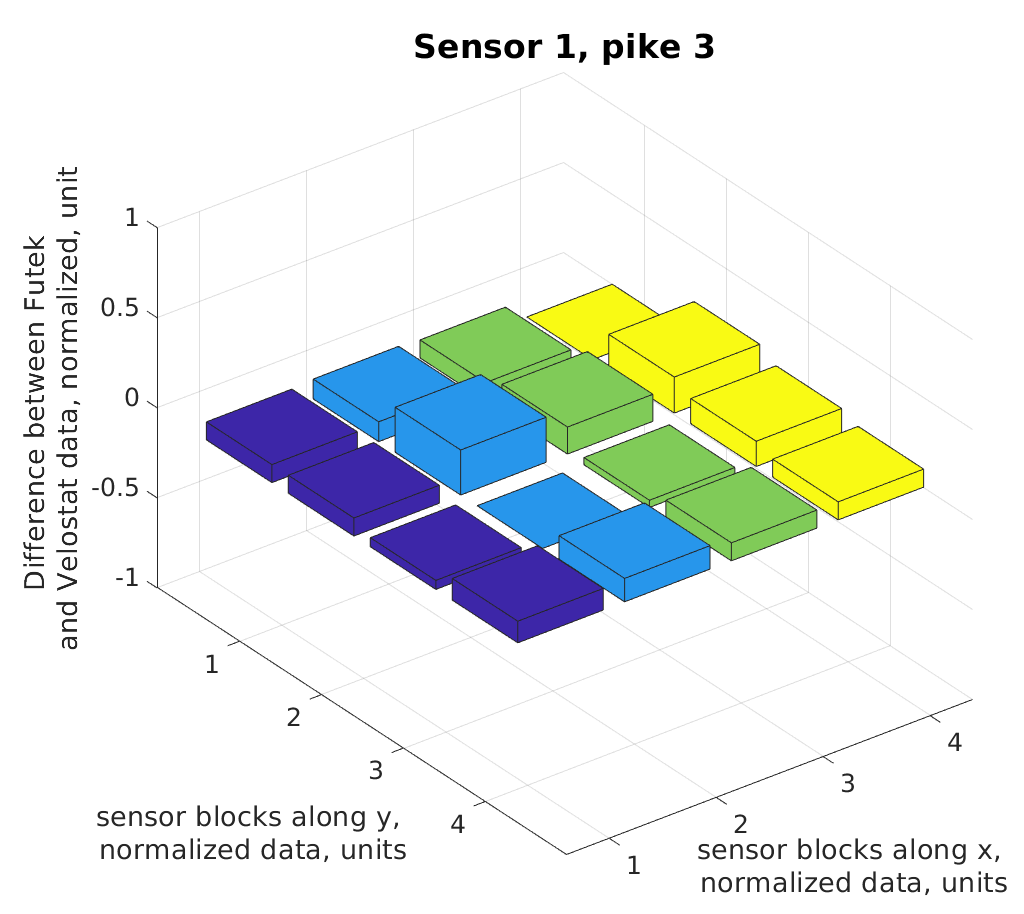
\includegraphics[height=5cm,width=1\textwidth,keepaspectratio]{sens1_pike3.png}
        \caption{Диаметр насадки равный 8 мм }
        \label{fig:sens1_pike3}
    \end{subfigure}
    \caption{Динамический эксперимент}
    \label{fig:dynamics_exp}
\end{figure}

По результатам исследований показано, что характеристики преобразователя удовлетворяют требованиям к системе тактильного восприятия шагающего робота, когда ожидаемый размер площади контакта превышает 25 процентов площади преобразователя.